\subsection{Area of a Disc of Radius $r$}

\begin{tcolorbox}[title=Problem 3, breakable]
    (a) Suppose that the sides of a rectangles $S$ have lengths 
        $r$ and $s$. What are the lengths of the sides  of the 
        rectangle $F_{a, b}(S)$, i.e. of the rectangle obtained 
        by the mixed dilation $F_{a, b}$?

    (b) What is the area of $F_{a, b}$?

    (c) If $S$ is a bounded region in the plane with area $A$,
        what is the area of $F_{a, b}(S)$?
\end{tcolorbox}

\textbf{Solution (a):}
\[F_{a, b}(S) \text{ has } ar \text{ width and } bs \text{ height.}\]
\textbf{Solution (b):}
\[\text{area}= ar \cdot bs = ab(rs)\]
\textbf{Solution (c):}
\[F_{a, b}(S) = ab(A)\]

\begin{tcolorbox}[title=Problem 4, breakable]
    (a) Show that the set of points $(u, v)$ satisfying the equation
        \[\left(\frac{u}{a}\right)^2 + \left(\frac{v}{b}\right)^2 = 1\]
        is the image of the circle of radius $1$ centered at $O$ under 
        the map $F_{a, b}$.

    (b) Let $a = 3$ and $b = 2$. Sketch this set, which is called an 
        \textbf{ellipse}.

    (c) Can you guess and motivate your guess as to what the area of the 
        region bounded by the ellipse in $(a)$ should be.
\end{tcolorbox}

\begin{proof}
    Let $C$ be the set of points making up the circle with radius $r = 1$ and center $O$.
    Let $P$ be an arbitrary point in $C$. Since $r = 1$, $d(O, P) = 1$.
    Let $L_1$ and $L_2$ be the vertical and horizontal lines through $O$, respectively.
    Drop perpendiculars from $P$ to $L_1$ and $L_2$, 
        and let $Q$ and $R$ be the feet of these perpendiculars on $L_1$ and $L_2$, respectively.
    Then $\triangle OQR$ is a right triangle with hypotenuse $\overline{OP}$, 
        and legs $\overline{OQ}$ and $\overline{OR}$ lying along $L_1$ and $L_2$.
    Let $u = d(OQ), v = d(OR)$ and by Pythagoras' Theorem $u^2 + v^2 = 1$.
    By applying the mapping $F_{a, b}$ to $\overline{OQ}, \overline{OR}$ 
        lengths $u, v$ are scaled by $\frac{1}{a}, \frac{1}{b}$ respectively
        we get $\left(\frac{u}{a}\right)^2 + \left(\frac{v}{b}\right)^2 = 1$.
\end{proof}

\textbf{Solution (b):}

\begin{figure}[h]
    \centering
    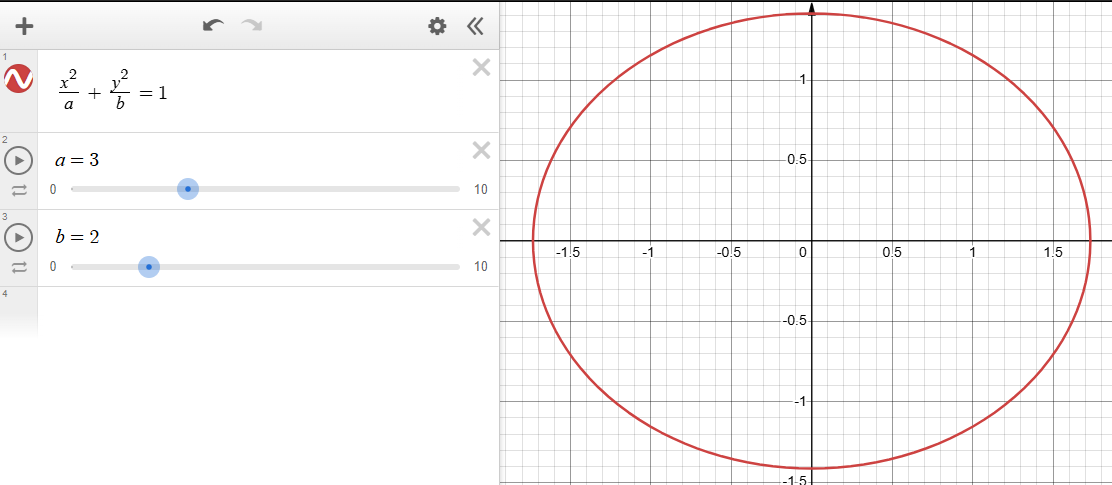
\includegraphics[width=0.6\textwidth]{images/ellipse.png}
\end{figure}

\textbf{Solution (c):}

Start with a circle of radius $r = 1$
    and suppose its area $A = \pi$.
We can subdivide this region into small squares with width $x$ and height $y$.
By Problem $3$ applying a $F_{a, b}$ to $x, y$ gives $ax, by$
    resulting in an area of $ab(xy)$.
Applying these dilations to the entire unit circle gives $ab\pi$.

\begin{tcolorbox}[title=Problem 7, breakable]
    Write up a discussion of how to give coordinates $(x, y, z)$ to 
    a point in $3-$space. In terms of these coordinates, what would the 
    effect of dilation by $r$?
\end{tcolorbox}

\textbf{Solution:}

Let $L_1, L_2, L_3$ be perpendicular lines intersecting at a point $O$.
Let $P$ be an arbitrary point in space.
Let the distances of the segments formed by dropping perpendiculars
    from $P$ to $L_1, L_2, L_3$ on one side be $(x, y, z)$.
On the opposite side, they are $(-x, -y, -z)$.

Let $V$ be the volume of a region in $3$-space. The effect of 
a dilation by $r$ would be to multiply the volume by $r^3$, giving $r^3 V$.

\begin{tcolorbox}[title=Problem 8, breakable]
    Generalize the discussion of this section to the $3$-dimensional
    case. Specifically:

    (a) Under dilation by $r$, how does the volume of a cube change?

    (b) How does the volume of a rectangle box with sides $a, b, c$ change?
        Draw a picture, say $r = \frac{1}{2}, r = 2, r = 3$, arbitrary $r$.

    (c) How would the volume of a $3-$dimensional solid change under 
        dilation by $r$?

    (d) The volume of the solid ball of radius $1$ in $3-$space is equal 
        to $\frac{4}{3} \pi$. What is the volume of the ball of radius 
        $r$ in $3-$space?
\end{tcolorbox}

\textbf{Solution (a):}

Under dilation $r$ the new volume $V' = r^3 V$ where $V$ is the volume 
    of the original cube.

\textbf{Solution (b):}

\begin{figure}[h]
    \centering
    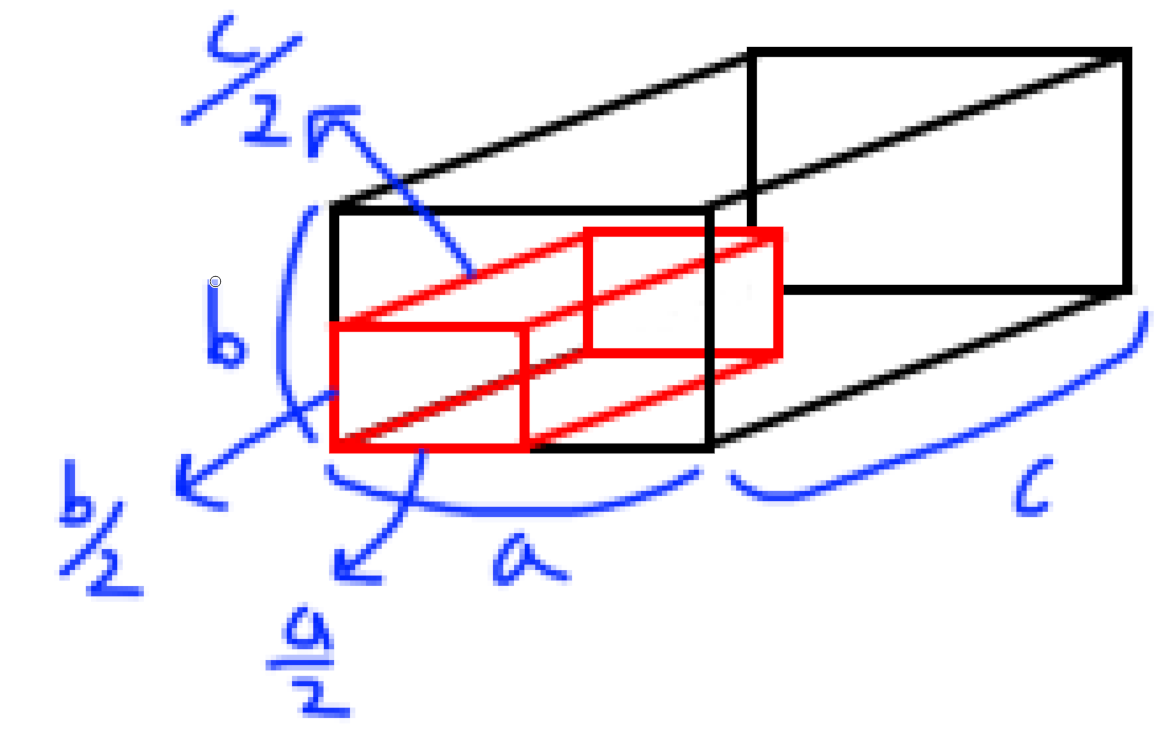
\includegraphics[width=0.6\textwidth]{images/half_rect.png}
\end{figure}

\begin{figure}[h]
    \centering
    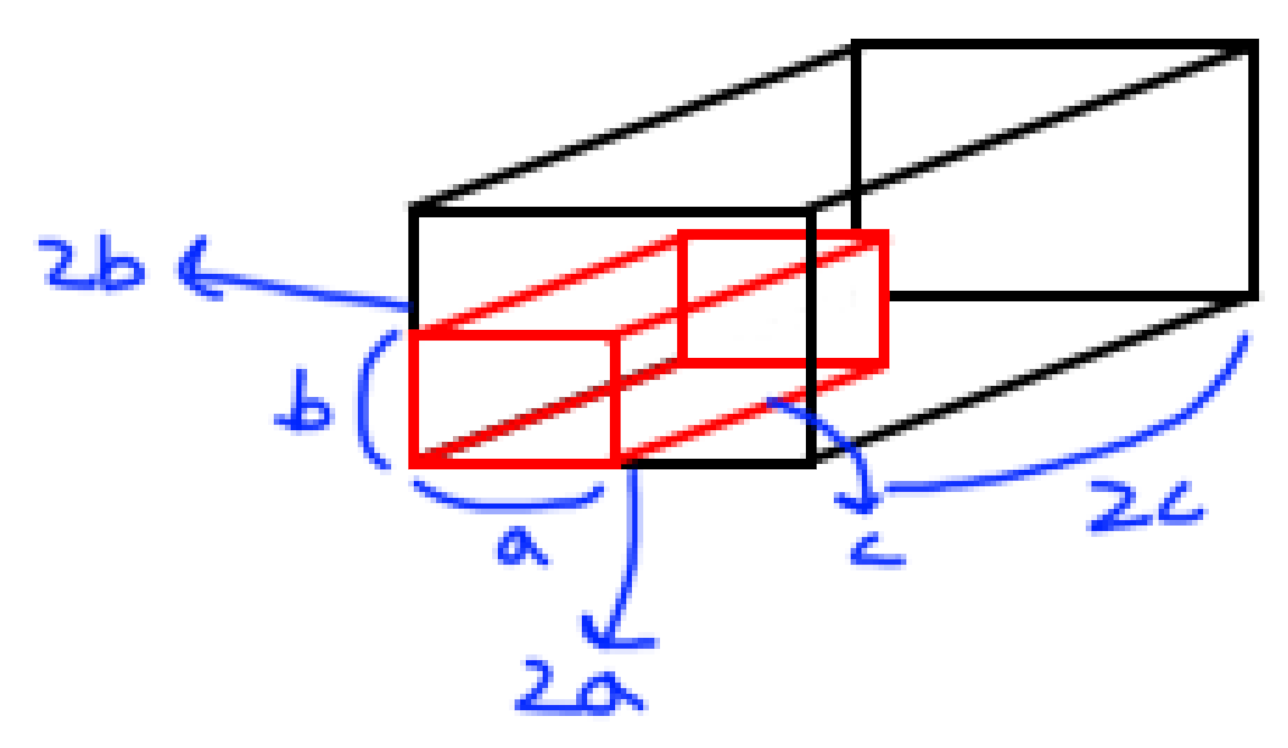
\includegraphics[width=0.6\textwidth]{images/2_rect.png}
\end{figure}

\begin{figure}[h]
    \centering
    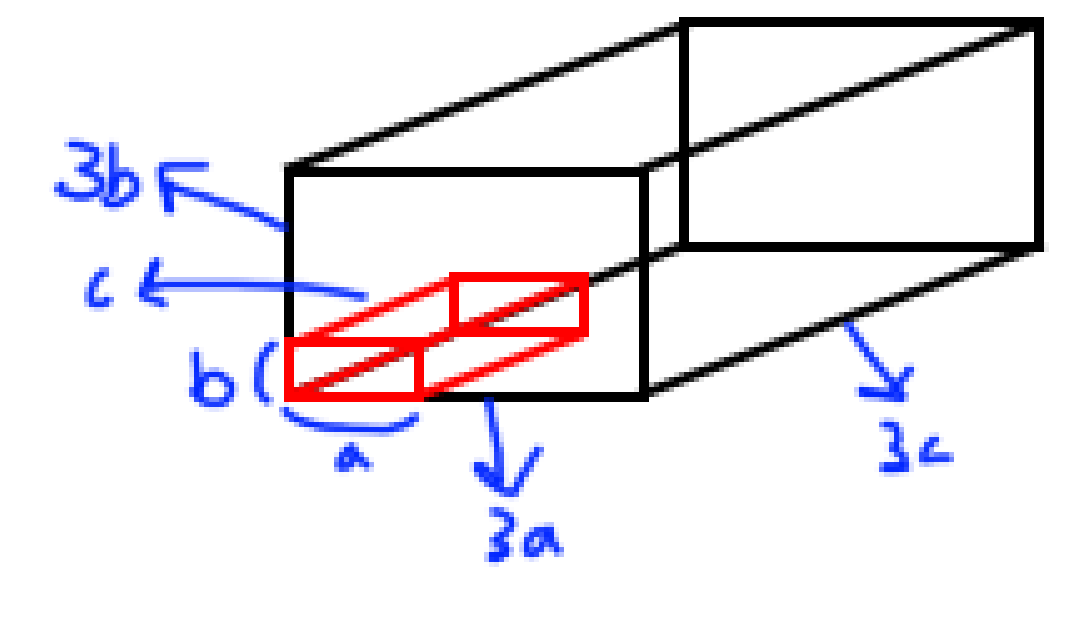
\includegraphics[width=0.6\textwidth]{images/3_rect.png}
\end{figure}

There are three cases for an arbitrary $r$ shown below
    depending on if $r < 1, r = 1, r > 1$.
If $r = 1$ the rectangle doesn't change that image isn't shown.
The first image shows if $r < 1$ and the second shows if $r > 1$.

\begin{figure}[h]
    \centering
    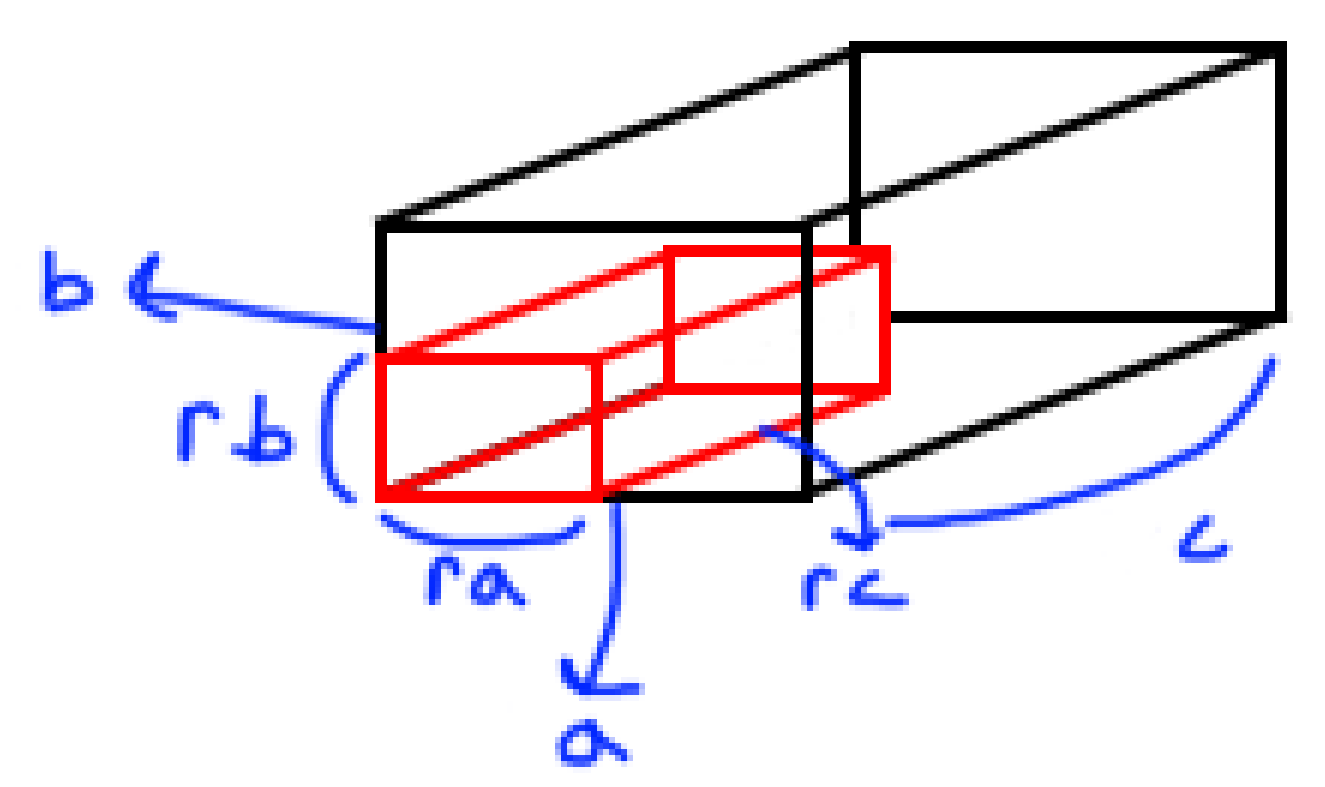
\includegraphics[width=0.6\textwidth]{images/arb1_rect.png}
\end{figure}

\begin{figure}[h]
    \centering
    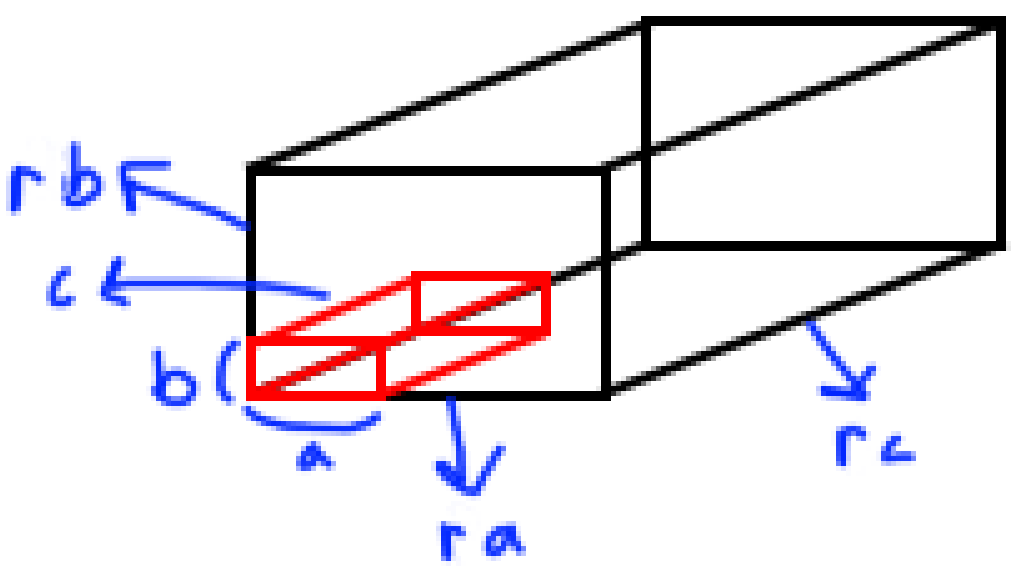
\includegraphics[width=0.6\textwidth]{images/arb2_rect.png}
\end{figure}

\textbf{Solution (c):}

Let $V$ be the volume of a solid. Under dilation $r$ the volume of the 
new solid is 
\[r^3 \cdot V\]

\textbf{Solution (d):}

\[V = r^3 \cdot \frac{4}{3}\pi\]

\begin{tcolorbox}[title=Problem 9, breakable]
    Write down the equation of a sphere of radius $r$ centered at the 
    origin in $3-$space.
\end{tcolorbox}

\textbf{Solution:}
\[a^2 + b^2 + c^2 = r^2\]

\begin{tcolorbox}[title=Problem 10, breakable]
    How would you define the volume of a rectangle solid whose sides 
    have lengths $a, b, c$.
\end{tcolorbox}

\begin{definition}
    Let the volume $V$ of a rectangle $R$ be defined as
    \[V = a \cdot b \cdot c\]
\end{definition}

\begin{tcolorbox}[title=Problem 11, breakable]
    Let $a, b, c$ be positive numbers. Let $\mathbb{R}^3$ be $3-$space,
    that is, the set of all triples of numbers $(x, y, z)$. Let 
    \[F_{a, b, c}: \mathbb{R^3} \rightarrow \mathbb{R}^3\]
    be the mapping
    \[(x, y, z) \rightarrow (ax, by, cz)\]
    Thus $F_{a, b, c}$ is a generalization to a $3-$space of our mixed 
    dilation $F_{a, b}$.

    (a) What is the image of a cube whose sides have length $1$ under $F_{a, b, c}$?
    
    (b) A rectangular box $S$ has sides of length $r, s, t$ respectively.
        What are the lengths of the sides of the image $F_{a, b}(S)$?
        What is the volume of $F_{a, b, c}(S)$?

    (c) Let $S$ be a solid in $3-$space, and let $V$ be its volume. 
        In terms of $V$, $a, b, c$ what is the volume of the image $S$
        under $F_{a, b, c}$?
\end{tcolorbox}

\textbf{Solution (a):}

The image of a cube whose sides have length $1$ under $F_{a, b, c}$
is a rectangular prism of side lengths $a, b, c$.

\textbf{Solution (b):}

The lengths of the sides of the image $F_{a, b}(S)$ is $ar, bs, t$.
The volume of $F_{a, b, c}(S)$ is $V = abc(rst)$.

\textbf{Solution (c):}

Let $V'$ be the volume of the image.
\[V' = abc V\]

\begin{tcolorbox}[title=Problem 12, breakable]
    What is the volume of the solid in $3-$space consisting of all points
    $(x, y, z)$ satisfying the inequality
    \[\left(\frac{x}{3}\right)^2 + \left(\frac{y}{2}\right)^2 + \left(\frac{z}{7}\right)^2 \le 1\]
\end{tcolorbox}

\textbf{Solution:}
\[V = 3 \cdot 2 \cdot 7 \cdot \frac{4}{3} \pi\]

\begin{tcolorbox}[title=Problem 14, breakable]
    Let $a, b, c$ be numbers $>0$. What is the volume of the solid 
    in $3-$space consisting of all points $(x, y, z)$ satisfying
    the inequality
    \[\left(\frac{x}{a}\right)^2 + \left(\frac{y}{b}\right)^2 + \left(\frac{z}{c}\right)^2 \le 1\]
\end{tcolorbox}

\textbf{Solution:}
\[V = a \cdot b \cdot c \cdot \frac{4}{3} \pi\]

\begin{tcolorbox}[title=Problem 15, breakable]
    What about $4-$space? $n-$space for arbitrary $n$?
\end{tcolorbox}

Let $V'$ be volume of $4-$D sphere.
The volume of the solid 
    in $4-$space consisting of all points $(x, y, z, d)$ satisfying
    the inequality
\[\left(\frac{x}{a}\right)^2 + \left(\frac{y}{b}\right)^2 
+ \left(\frac{z}{c}\right)^2 + \left(\frac{p}{d}\right)^2 \le 1\]
has volume
\[V = a \cdot b \cdot c \cdot d \cdot V'\]

Let $V'$ be volume of $n-$D sphere.
The volume of the solid 
    in $n-$space consisting of all points $(x_1, x_2, x_3, \ldots, x_n)$ satisfying
    the inequality
\[\left(\frac{y_1}{x_1}\right)^2 + \left(\frac{y_2}{x_2}\right)^2 
+ \left(\frac{y_3}{x_3}\right)^2 + \ldots +  \left(\frac{y_n}{x_n}\right)^2 \le 1\]
has volume
\[V = x_1 \cdot x_2 \cdot x_3 \cdot \ldots \cdot x_n \cdot V'\]